\skriptsection{Complexe Funktionen (Abbildungen)}{37ff}
Eine complexe Funktion hat einen 2-dimensionalen Input ($z_1$, $z_2$) und einen
2-dimensionalen Output ($w_1$, $w_2$). \\
Diese Abbildungen sind bis jeweils auf wenige Punkte (bei der Sinus-Funktion
$\pm$1, etc) winkeltreu.\\
$ f: \mathbb{D} \subseteq \mathbb{C} \mapsto \mathbb{C} \qquad z  \mapsto w = f(z)$\\
$w_1 = \text{Re}(f(r+jc)); w_2 = \text{Im}(f(r+jc))$ 
 

\skriptsubsection{Lineare Funktion}{41ff}
  \begin{minipage}{9cm}
       $$ f : z \mapsto w = az + b \qquad (a, b \in \mathbb{C} \text{ und } a \neq0)\\$$
    - für $a = 1$ eine Translation um den Ortsvektor b \\
    - für $a \neq 1$ eine Drehstreckung mit dem Zentrum $\frac{b}{1-a}$, dem 
    Drehwinkel $\arg(a)$ und dem Streckfaktor $|a|$.  
    \end{minipage}
  \hspace{2cm}
  \begin{minipage}{8cm}
      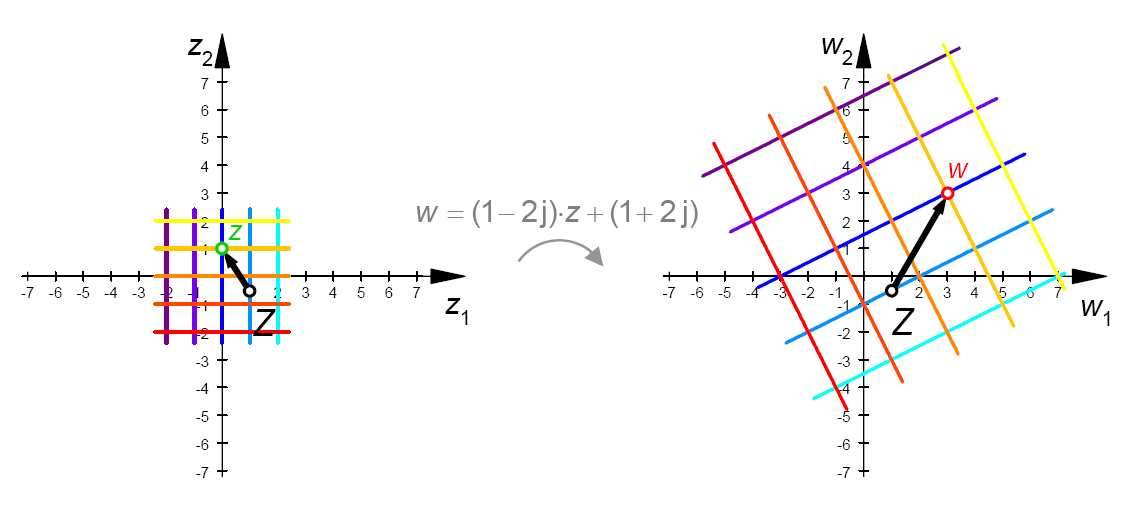
\includegraphics[width=8cm]{./bilder/LineareFunktion.png}
    \end{minipage}

\skriptsubsection{Quadratfunktion und Quadratwurzelfunktion}{45ff}
  \begin{minipage}{9cm}
      $$ f : z \mapsto w = z^2 \qquad \qquad f : z \mapsto w = \sqrt{z} $$\\
    Bei der Quadratfunktion wird schon die rechte Hälfte der z-Ebene auf die ganze
    w-Ebene abgebildet (die Argumente werden verdoppelt). Daraus ergibt sich
    zwei bzw. mehrere Ebenen.
    \end{minipage}
  \hspace{2cm}
  \begin{minipage}{8cm}
      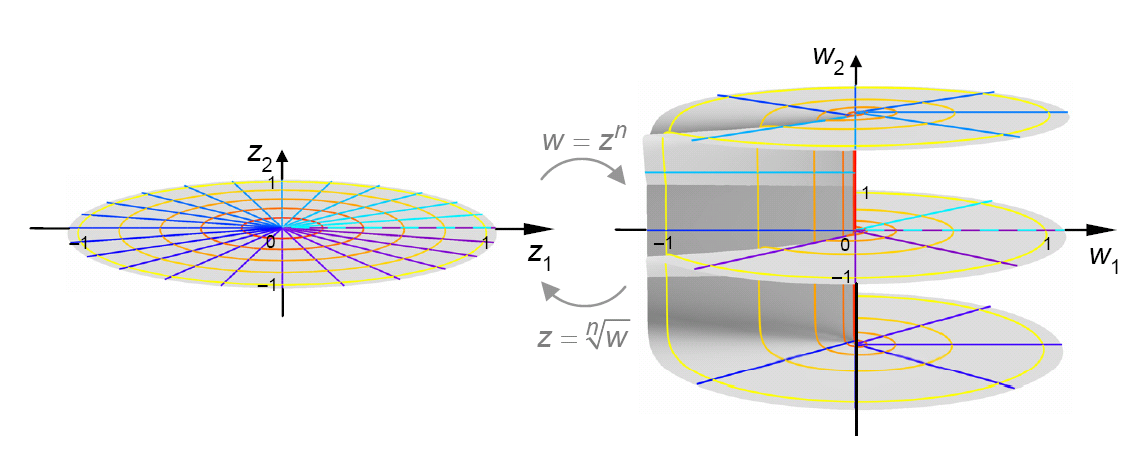
\includegraphics[width=8cm]{./bilder/RiemannischeFlaeche.png} 
      Eine Riemanische Fläche 3.Grades
    \end{minipage}

\skriptsubsection{Winkeltreue}{}
\skriptsubsubsection{differenzierbare Funktionen}{}
Eine komplexe differenzierbare Funktion $f$ ist in allen Punkten mit
$f'(z)\neq0$ eine winkeltreue Abbildung. Sie bewirkt dort lokal eine
Drehstreckung mit Drehwinkel $arg\left[f'(z)\right]$ und Streckfaktor
$\left|f'(z)\right|$

\skriptsubsubsection{quadratische Funktionen}{}
Die Quadratfunktion $f:Z\mapsto z^2$ bildet die $z$-Ebene bijektiv auf eine
zweiblättirge Riemamsche Fläche ab. Sie hat die Ableitungsfunktion
$f':z\mapsto 2z$ und ist deshalb überall ausser im Koordinatenursprung
winkeltreu.\\
Die Quardatwurzelfunktion $f^{-1}:w \mapsto \sqrt{w}$ ist somit ebenfals überall
ausser im Koordinaten ursprung winkelreu.

\skriptsubsection{Kehrwertfunktion und Kreisspiegelung}{51ff}
  $$ f : z \mapsto w = \frac{1}{z}; \quad (\arg(w) = -\arg(z), |w| = \frac{1}{|z|})
  \qquad \qquad 
  \overline{f}: z \mapsto w = \frac{1}{\overline{z}};  \quad  
  (\arg(w) = \arg(z), |w| = \frac{1}{|z|}) $$\\
  Kreisspiegelung: Alle Punkte auf der z-Ebene werden am Einheitskreis gespiegelt.
  Geraden auf Kreise abgebildet und umgekehrt. Der Ursprungspunkt (0;0) wird auf
  $ \infty $ abgebildet (auf allen Winkeln zwischen $0^o-360^o$). Die
  Abbildungen sind
  im verallgemeinerten Sinn (Geraden sind Kreise mit unendlichem Radius)
  kreistreu. Ausserdem sind sie bis auf den Koordinatenursprung winkeltreu\\
  \begin{minipage}{9cm}
    \begin{tabbing}
          xxxxxxxxxxxxxxxxxxxxxxx\=xxxxxxxxxxxxxxxxxxxxxxxx\kill
          - Gerade durch 0 $\Longrightarrow$ \>Fixgerade (gleiche Gerade, aber
          die \\ \>Punkte darauf sind anders verteilt)\\ \\
      - Gerade nicht durch 0 $\Longrightarrow$ Kreis durch 0\\ \\ \\ \\ \\ \\ \\ \\
      - Kreis nicht durch 0 $\Longrightarrow$ \>Spiegelung des Kreises\\ \> an dem
      Einheitskreis\\ \\
      - Kreis durch 0 $\Longrightarrow$\>Gerade nicht durch 0
        \end{tabbing}
  \end{minipage}
  \hspace{2cm}
  \begin{minipage}{6cm}
    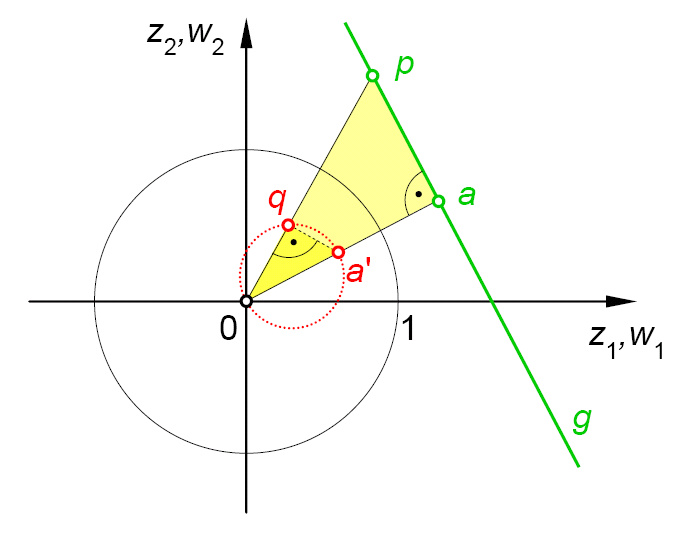
\includegraphics[width=6cm]{./bilder/GeradeKreisspiegelung.png} 
      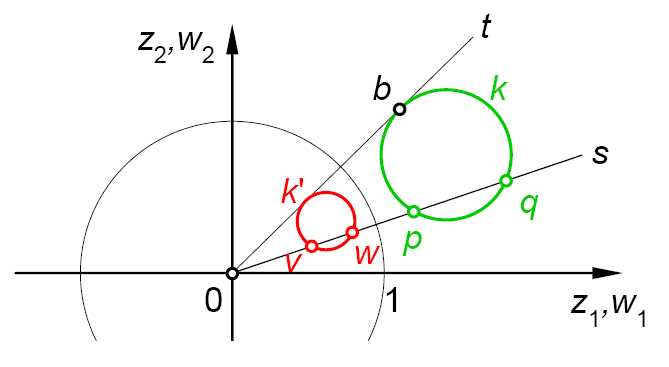
\includegraphics[width=6cm]{./bilder/KreisKreisspiegelung.png}
    \end{minipage}

\skriptsubsection{Möbiustransformation}{57ff}
  \begin{minipage}{10cm}
    $$ f : z \mapsto w = f(z) = \frac{az + b}{cz + d}$$
    $$(a, b, c, d \in 
    \mathbb{C} \text{ mit } c \neq 0 \text{ und } ad - bc \neq 0) $$
    Die Möbiustransformation ist eine Verkettung einer linearen Funktion, der Kehrwertfunktion und einer weiteren linearen Funktion. \\
    Diese Transformationen sind winkel- und kreistreu. Die Umkehrfunktion ergibt wieder eine Möbiustransformation. \\
    Eigentlich besitzt diese Funktion nur drei Parameter da man den Bruch
    $\frac{az + b}{cz + d}$ stets so kürzen kann dass einer der vier Parameter 1
    ist. Durch die 3 Freiheitsgrade kann man unterschiedlichste kriterien
    vorgeben und damit komplizierte Umformungen machen, wie im Bild gezeigt wird:
  
  \end{minipage}
  \hspace{2cm}
  \begin{minipage}{7cm}
    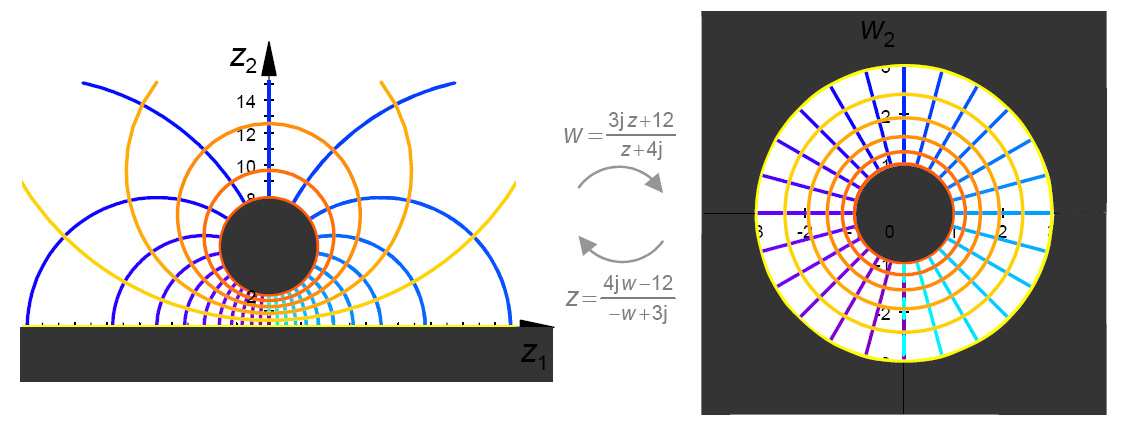
\includegraphics[width=7cm]{./bilder/Moebiustransformation.png} 
  \end{minipage}

\skriptsubsection{Joukowski-Funktion}{60ff}
  \begin{minipage}{10cm}
    $$ f : z \mapsto w = z + \frac{1}{z}  $$
    Die Funktion ist winkeltreu bis auf $\pm$2\\
    Wenn man einen Kreis, der nicht ganz im Zentrum steht transformiert ergibt
    sich ein Flügelprofil
  \end{minipage}
  \hspace{2cm}
  \begin{minipage}{7cm}
    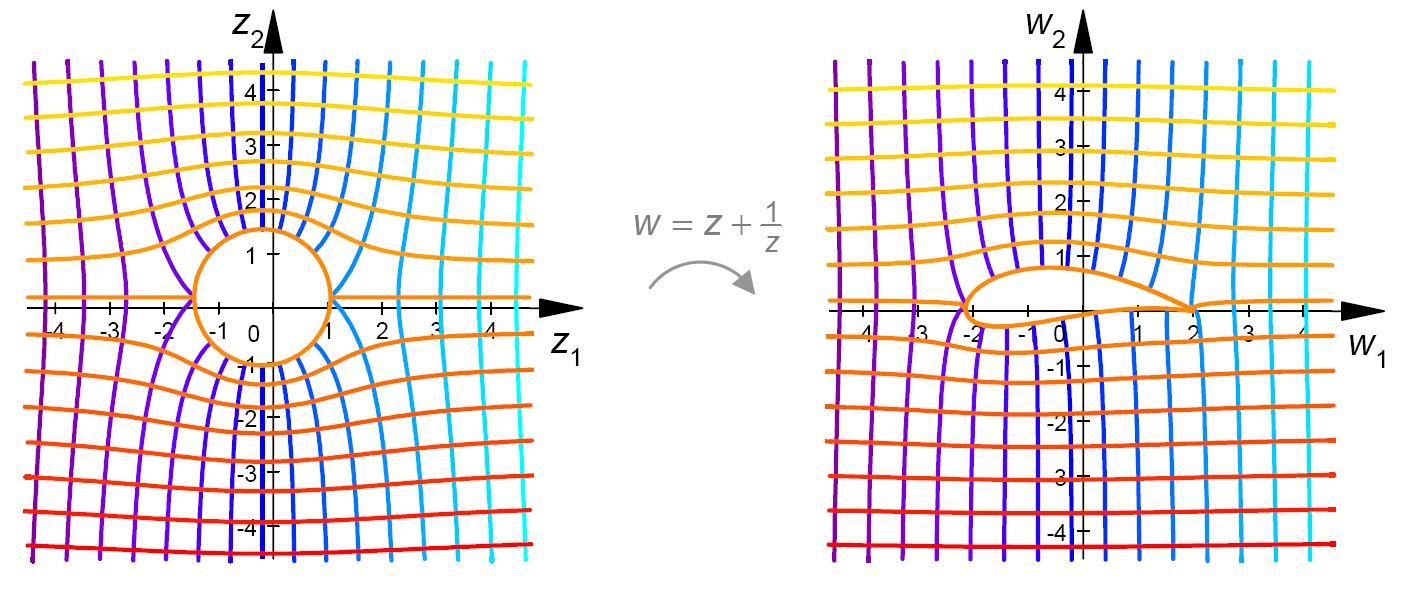
\includegraphics[width=7cm]{./bilder/joukowskiFunktion.png} 

  \end{minipage}
\skriptsubsection{Exponentialfunktion}{64ff} 
  \begin{minipage}{9cm}
    $$ f : z \mapsto w = e^z $$
    Waagrechte Gitternetzlinen gehen gemäss der obigen Gleichung in Strahlen
    über, die im Koordinatenursprung beginnen, senktrechte Gitternetzlinien in
    Kreise um den Koordinatenursprung. Die e$^z$-Funktion ist periodisch, deshalb
    braucht es eine Riemansche Fläche\\ \\
    Mit dieser Funktion kann man das Feld bei den Rändern des Plattenkondensator
    berechnen 
  \end{minipage}
  \hspace{2cm}
  \begin{minipage}{7cm}
    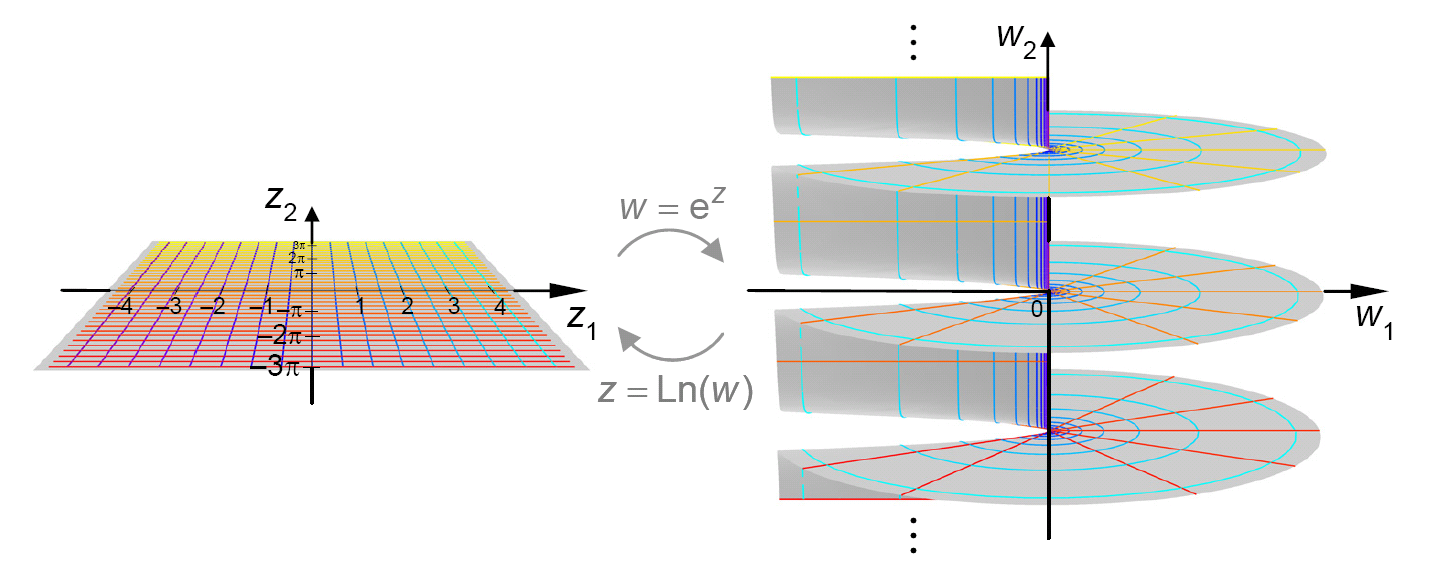
\includegraphics[width=7cm]{./bilder/ehochz.png} 
    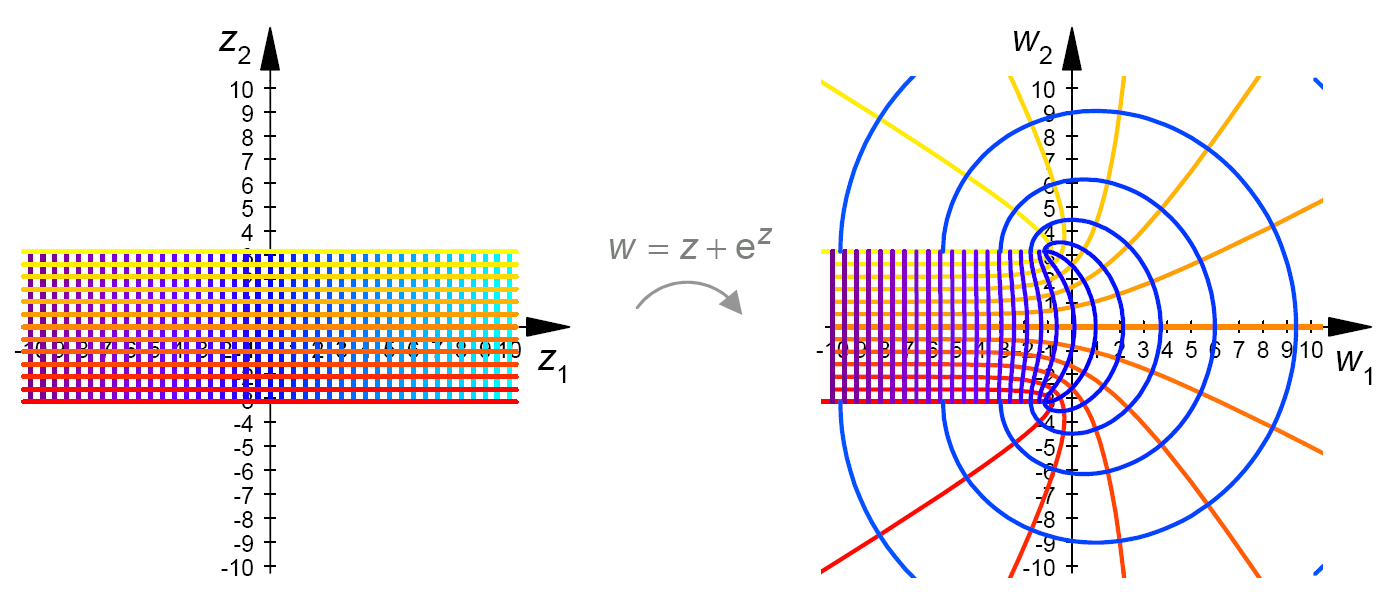
\includegraphics[width=8cm]{./bilder/plattenkondensator.png}    
  \end{minipage}

\skriptsubsection{Sinus-Funktion}{67f}
   \begin{minipage}{10cm}
    $$ f : z \mapsto w = \sin(z) $$    
    Die Sinusfunktion ist ausser bei den Punkten $z = \frac{\pi}{2}+ k\pi (k \in
    \mathbb{Z}))$ winkeltreu
  \end{minipage}
  \hspace{2cm}
  \begin{minipage}{7cm}
    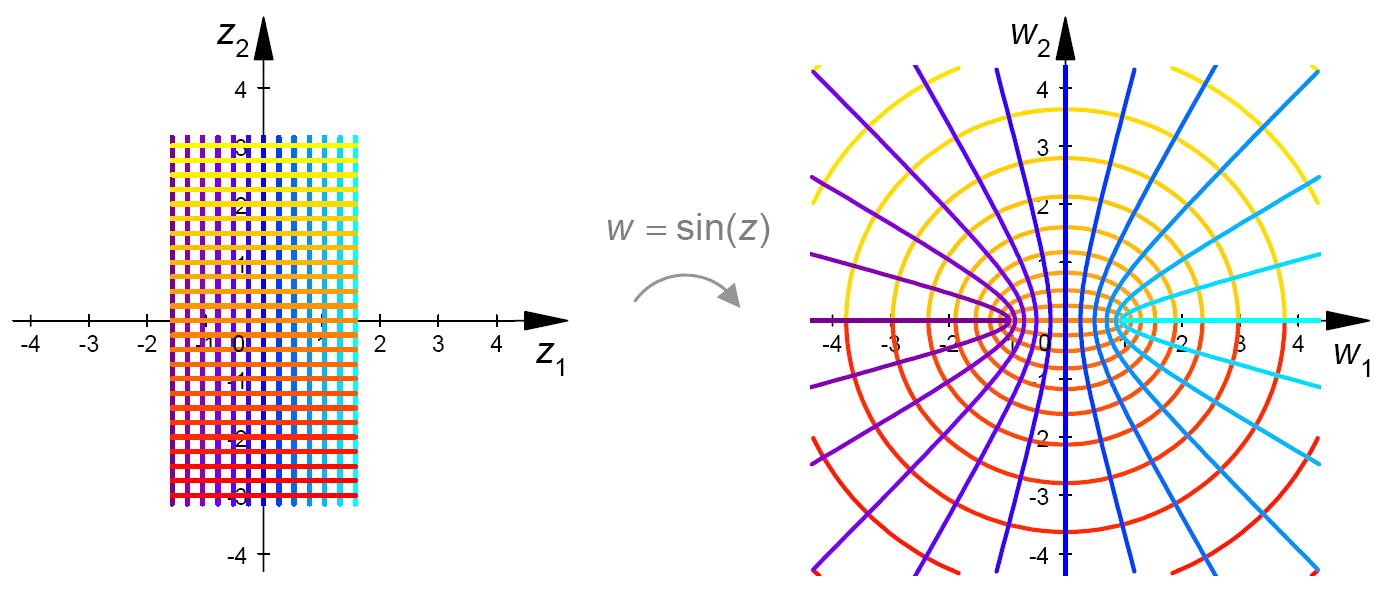
\includegraphics[width=7cm]{./bilder/sinus.png} 
  
  \end{minipage}
 
\subsection{Kreisgleichung}
Die Lösungen von z bilden einen Kreis in der mit dem Radius $r$ um den Mittelpunkt $M=(m_x, m_y) \Rightarrow m=m_x + j m_y$. \\
$$|z-m| = r; \qquad 
(z-m)(\overline{z} - \overline{m}) = r^2; \qquad 
z\overline{z} - \overline{m}z - m\overline{z} + m\overline{m} = r^2$$
$$ \text{Parameterform: } f(t) = m + r \cdot e^{jt}, \quad \text{mit } (0 \leq t \leq 2 \pi) $$

